\documentclass[12pt,letterpaper]{article}

\usepackage{amsfonts}
\usepackage{graphics}
\usepackage{graphicx}
\usepackage{colortbl}
\usepackage{amsmath}

\newenvironment{proof}{\noindent{\bf Proof:}}{\qed\bigskip}

\newtheorem{theorem}{Theorem}
\newtheorem{corollary}{Corollary}
\newtheorem{lemma}{Lemma} 
\newtheorem{claim}{Claim}
\newtheorem{fact}{Fact}
\newtheorem{definition}{Definition}
\newtheorem{assumption}{Assumption}
\newtheorem{observation}{Observation}
\newtheorem{example}{Example}
\newcommand{\qed}{\rule{7pt}{7pt}}

\newcommand{\assignment}[4]{
\thispagestyle{plain} 
\newpage
\setcounter{page}{1}
\noindent
\begin{center}
\framebox{ \vbox{ \hbox to 6.28in
{\bf CS578/STAT590: Introduction Machine Learning \hfill #1}
\vspace{4mm}
\hbox to 6.28in
{\hspace{2.5in}\large\mbox{Problem Set #2}}
\vspace{4mm}
\hbox to 6.28in
{{\it Handed Out: #3 \hfill Due: #4}}
}}
\end{center}
}

\newcommand{\solution}[4]{
\thispagestyle{plain} 
\newpage
\setcounter{page}{1}
\noindent
\begin{center}
\framebox{ \vbox{ \hbox to 6.28in
{\bf CS578/STAT590: Introduction to Machine Learning \hfill #4}
\vspace{4mm}
\hbox to 6.28in
{\hspace{2.5in}\large\mbox{Problem Set #3}}
\vspace{4mm}
\hbox to 6.28in
{#1 \hfill {\it Handed In: #2}}
}}
\end{center}
\markright{#1}
}

\newenvironment{algorithm}
{\begin{center}
\begin{tabular}{|l|}
\hline
\begin{minipage}{1in}
\begin{tabbing}
\quad\=\qquad\=\qquad\=\qquad\=\qquad\=\qquad\=\qquad\=\kill}
{\end{tabbing}
\end{minipage} \\
\hline
\end{tabular}
\end{center}}

\def\Comment#1{\textsf{\textsl{$\langle\!\langle$#1\/$\rangle\!\rangle$}}}



\oddsidemargin 0in
\evensidemargin 0in
\textwidth 6.5in
\topmargin -0.5in
\textheight 9.0in

\begin{document}

\solution{Gen Nishida}{\today}{2}{Fall 2014}
% Fill in the above, for example, as follows:
% \solution{John Smith}{\today}{1}{Fall 2014}

\pagestyle{myheadings}  % Leave this command alone

\section{Questions}

\begin{enumerate}
\item Given $n$ boolean variables $(x_1,\cdots,x_n)$, we define our target classification function $f(\cdot)$ as $f(\cdot)=1$ if at least 3 variables are active. For $n=5$ show how this function can be represented as (1) Boolean function (2) Linear function.

(1) Boolean function

By using conjunctions for every combination of three variables, we can test if at least three variables are active. Therefore, the Boolean function for this can be represented as follows:
\begin{eqnarray*}
f=(x_1 \wedge x_2 \wedge x_3) \vee (x_1 \wedge x_2 \wedge x_4) \vee (x_1 \wedge x_2 \wedge x_5) \vee (x_1 \wedge x_3 \wedge x_4) \vee (x_1 \wedge x_3 \wedge x_5) \\
\vee (x_1 \wedge x_4 \wedge x_5) \vee (x_2 \wedge x_3 \wedge x_4) \vee (x_2 \wedge x_3 \wedge x_5) \vee (x_2 \wedge x_4 \wedge x_5) \vee (x_3 \wedge x_4 \wedge x_5)
\end{eqnarray*}

(2) Linear function

The equivalent linear function just needs to check whether the sum is more than two. Thus,
\[
f = {\rm sign}(x_1 + x_2 + x_3 + x_4 + x_5 - 2)
\]
where
\[
{\rm sign}(x) = \begin{cases}
1 & ({\rm if} \; x > 0) \\
0 & Otherwise
\end{cases}
\]


\item Let $CON_B$ be the set of all different monotone conjunctions defined over $n$ boolean variables. What is the size of $CON_B$?

For every variable, there are two cases, active or not active. Thus, the size of $CON_B$ is $2^n$. 

\item Let $CON_L$ be the set of all linear functions defined over $n$ boolean variables that are consistent with the functions in $CON_B$. What is the size of $CON_L$?

Given a monotone conjunction, one example of the equivalent linear functions is defined by the sign of the summation of all the active literals subtracted by (the number of the active literals - 1). For instance, for a monotone conjunction $f_b = x_1 \wedge x_3 \wedge x_5$, the corresponding linear function is $f_l = {\rm sign}(x_1 + x_3 + x_5 - 2)$. However, the linear function can have any real nubmer as the coefficient of each literal. In the above case, for instance, another equivalent linear function would be $f_l^\prime = {\rm sign}(2 x_1 + 2 x_3 + 2 x_5 - 4)$, and both $f_l$ and $_l^\prime$ are consistent with $f_b$. Thus, the size of $CON_L$ is inifinite.

\item Define in one sentence: Mistake bound.

Mistake bound is the maximum number of mistakes that can be made by an online learning algorithm, which is also used to evaluate the performance of the convergence of the algorithm. 

\item Suggest a mistake bound algorithm for learning Boolean conjunctions. Show that your algorithm is a mistake bound algorithm for Boolean conjunctions.

Algorithm 1 shows the mistake bound algorithm for learning Boolean conjunctions.

\begin{algorithm}
\caption{Mistake bound algorithm for learnign Boolean conjunctions}\label{euclid}
\begin{algorithmic}[1]
\Procedure{LearnBooleanConjunctions()}{}
\State Initialize the hypothesis: $h =  x_1 \wedge \neg x_1 \wedge x_2 \wedge \neg x_2 \wedge \cdots \wedge x_n \wedge \neg x_n$
\ForAll{examples $x \in X$}
\If{$h(x) \neq y$}
\State eliminate literals that are not active (0) \hspace*{\fill} (See some examples in Figure \ref{fig:learning_process})
\EndIf
\EndFor
\EndProcedure
\end{algorithmic}
\end{algorithm}



An example of the learning process is shown in Figure \ref{fig:learning_process}. When the first mistake is made for an training data $x=(1, 0, 0)$, the literals $\neg x_1$, $ x_2$, and $x_3$ are not active, and these literals are removed from the conjunctions, which results in the updated hypothesis $h = x_1 \wedge \neg x_2 \wedge \neg x_3$. 

For every mistake, we remove at least one unnecessary literal from the conjunctions. Since we have $2n$ literals at the beginning, and at least one literal in the conjunctions will be remained in the end, the total number of mistakes is at most $2n-1$, which is $O(n)$. Thus, this is a mistake bound algorithm.

\begin{figure}[hbtp]
\centering
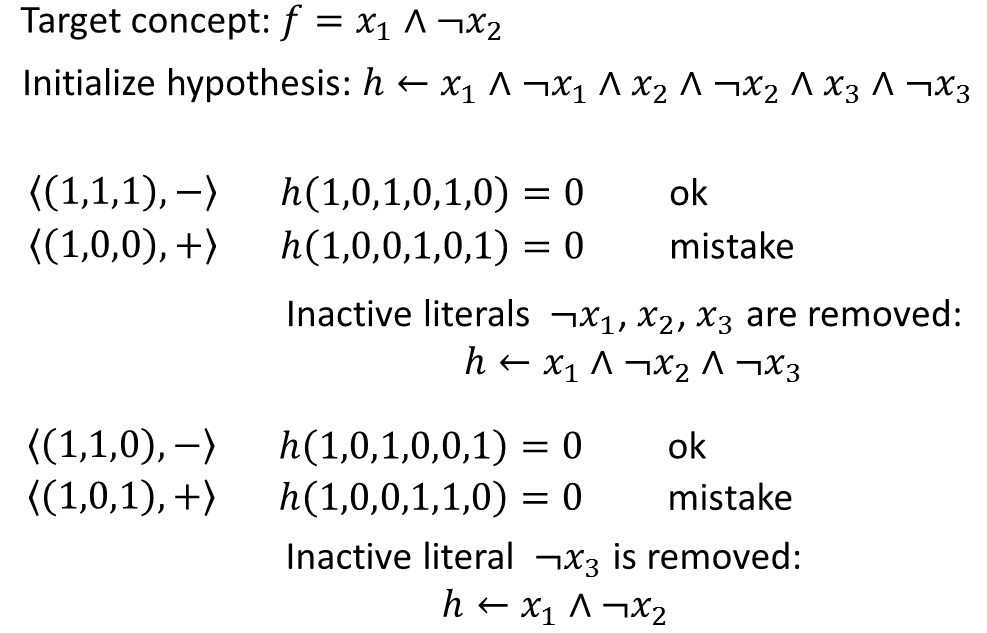
\includegraphics[width=100mm]{learning_process.jpg}
\caption{An example of a learning process}
\label{fig:learning_process}
\end{figure}

\item Given a linearly separable dataset consisting of 1000 positive examples and 1000 negative examples, we train two linear classifier using the perceptron algorithm. We provide the first classifier with a sorted dataset in which all the positive examples appear first, and then the negative examples appear. The second classifier is trained by randomly selecting examples at each training iteration.

(1) Will both classifiers converge?

Yes. For the linearly separable dataset, it is proved that the perceptron algorithm will converge, and the mistake bound is $R^2/\gamma^2$, which is independent from the order of the examples.

(2) What will be the training error of each one of the classifiers?

When both classifiers converge, no more mistakes will be made. In other words, the training error will be zero for both classifiers.

\item We showed in class that using the Boolean kernel function $K(x, y)=2^{same(x,y)}$ we can express all conjunctions over the attributes of $x$ and $y$ (with both the positive and negative literals). This representation can be too expressive. Suggest a kernel function $K(x, y)$ that can express all conjunctions of size at most $k$.

Every active conjunctions of size at most $k$ is a combination of positive or negative literals $l_i \in L$ that have the same value in $x$ and $y$ (i.e. $|L|=same(x,y)$). Then, counting the active conjunctions of size at most $k$ is reduced to selecting a set of literals of size at most $k$ from $L$. Thus,

\[
K(x, y)={}_{same(x,y)} C _0 + {}_{same(x,y)} C _1 + {}_{same(x,y)} C _2 + \cdots + {}_{same(x,y)} C _k
\]

\end{enumerate}

\section{Programming Assignment}


The learning results for $featrueSet=1$ is shown in Figure \ref{fig:F1_curve_1}.  The best F1 on the validation data was achieved when $maxIterations=438$. Since F1 score is a good gauge to measure the performance, I picked $maxIterations = 438$ that achieves the highest F1 score, and evaluate the performance (Table 1).

\begin{table}[htb]
\centering
  \begin{tabular}{|c|r|r|r|r|} \hline
    data & accuracy & precision & recall & F1 \\ \hline
    Training data & 0.87 & 0.94 & 0.75 & 0.83 \\ \hline
    Validation data & 0.93 & 0.92 & 0.92 & 0.92 \\ \hline
    Test data & 0.56 & 0.56 & 0.53 & 0.54 \\ \hline
  \end{tabular}
  \caption{The performace for $featureSet = 1$ and $maxIterations = 438$}
\end{table}

\begin{figure}[hbtp]
\centering
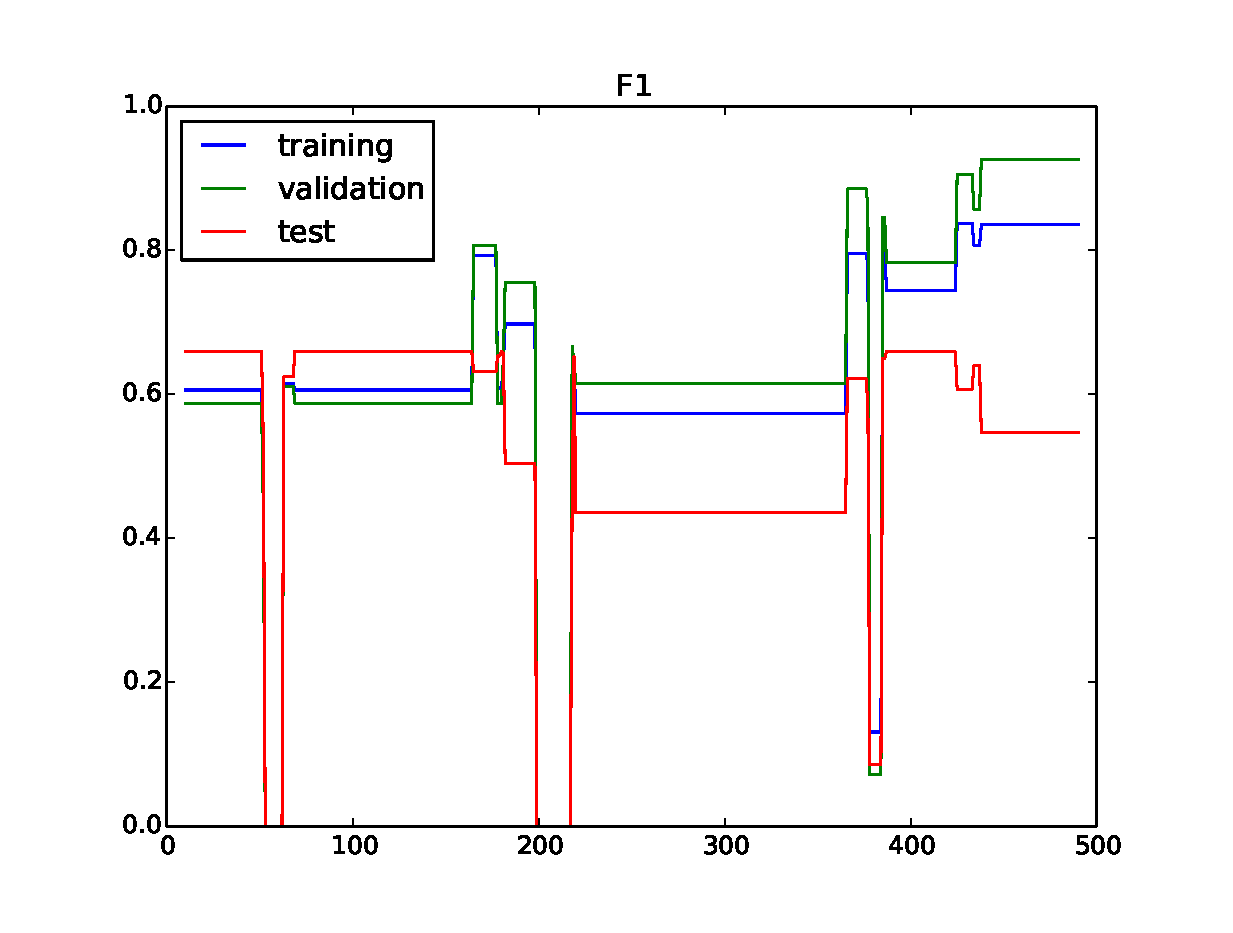
\includegraphics[width=100mm]{F1_curve_1}
\caption{F1 evolution over the number of examples for $featureSet=1$}
\label{fig:F1_curve_1}
\end{figure}

The learning results for $featrueSet=2$ is shown in Figure \ref{fig:F1_curve_2}. The best F1 on the validation data was achieved when $maxIterations=432$, and for the same reason, I picked $maxIterations = 432$ that achieves the highest F1 score, and evaluate the performance (Table 2).

\begin{table}[htb]
\centering
  \begin{tabular}{|c|r|r|r|r|} \hline
    data & accuracy & precision & recall & F1 \\ \hline
    Training data & 0.90 & 0.91 & 0.85 & 0.88 \\ \hline
    Validation data & 0.96 & 0.93 & 1.0 & 0.96 \\ \hline
    Test data & 0.57 & 0.55 & 0.69 & 0.61 \\ \hline
  \end{tabular}
  \caption{The performace for $featureSet = 2$ and $maxIterations = 432$}
\end{table}

\begin{figure}[hbtp]
\centering
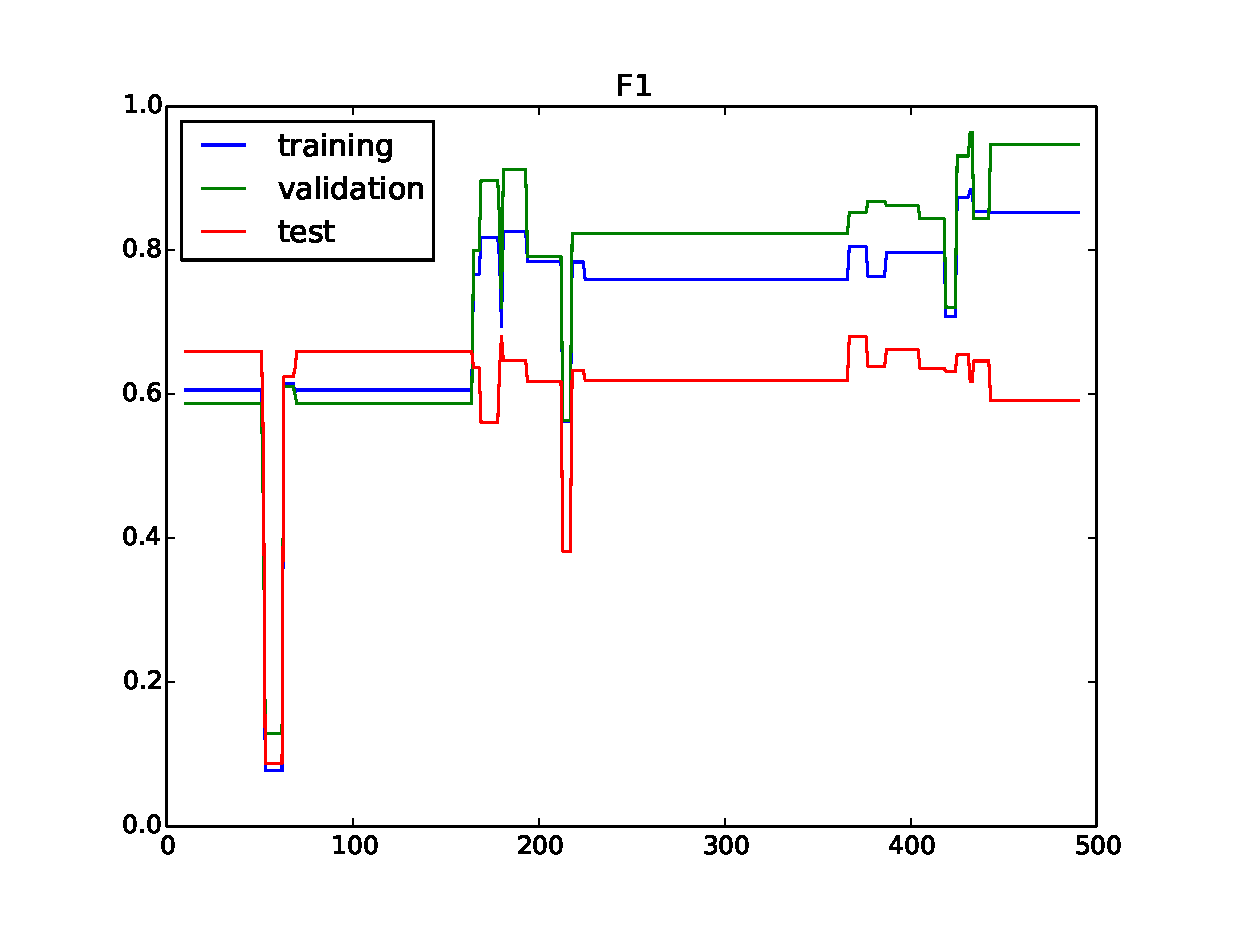
\includegraphics[width=100mm]{F1_curve_2}
\caption{F1 evolution over the number of examples for $featureSet=2$}
\label{fig:F1_curve_2}
\end{figure}

The learning results for $featrueSet=3$ is shown in Figure \ref{fig:F1_curve_3}. The best F1 on the validation data was achieved when $maxIterations=425$, and its performance is shown in Table 3.

\begin{table}[htb]
\centering
  \begin{tabular}{|c|r|r|r|r|} \hline
    data & accuracy & precision & recall & F1 \\ \hline
    Training data & 0.92 & 0.89 & 0.94 & 0.91 \\ \hline
    Validation data & 0.96 & 0.93 & 1.0 & 0.96 \\ \hline
    Test data & 0.52 & 0.50 & 0.81 & 0.62 \\ \hline
  \end{tabular}
  \caption{The performace for $featureSet = 3$ and $maxIterations = 425$}
\end{table}

\begin{figure}[hbtp]
\centering
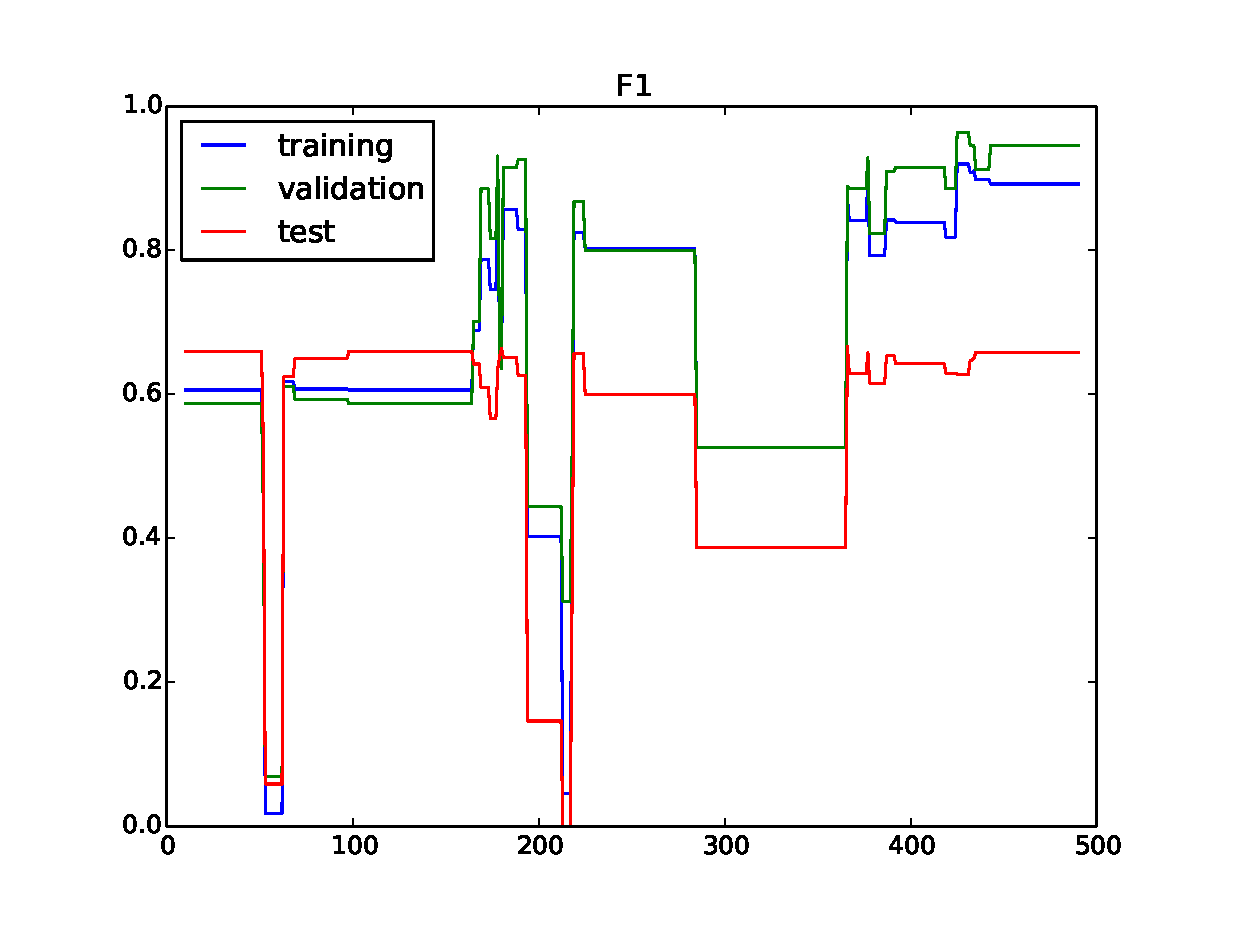
\includegraphics[width=100mm]{F1_curve_3}
\caption{F1 evolution over the number of examples for $featureSet=3$}
\label{fig:F1_curve_3}
\end{figure}

The results show the significant improvement in the performance by using more complex feature set (i.e. $featureSet = 2$ or $featureSet = 3$). Notice that the performance on the test data is also improved by using complex feature set without overfitting. This indicates that the linear function helps to keep the hypothesis from being overfitting even if we use a comples feature set.

\end{document}

